\ifx\boi\undefined\ifx\problemname\undefined
\providecommand\sampleinputname{}
\providecommand\sampleoutputname{}
\documentclass[russian]{templates/boi}
\problemlanguage{.ru}
\fi
\newcommand{\boi}{Балтийская Олимпиада по Информатике}
\newcommand{\practicesession}{Тренировочный раунд}
\newcommand{\contestdates}{27 апреля - 1 мая, 2018}
\newcommand{\dayone}{День 1}
\newcommand{\daytwo}{День 2}
\newcommand{\licensingtext}{Задача публикуется под лицензией CC BY-SA 4.0.}
\newcommand{\problem}{Задача}
\newcommand{\inputsection}{Ввод}
\newcommand{\outputsection}{Вывод}
\newcommand{\interactivity}{Интерактивность}
\newcommand{\grading}{Оценивание}
\newcommand{\scoring}{Очки}
\newcommand{\constraints}{Ограничения}
\renewcommand{\sampleinputname}{Пример ввода}
\renewcommand{\sampleoutputname}{Пример вывода}
\newcommand{\sampleexplanation}[1]{Объяснение примера #1}
\newcommand{\sampleexplanations}{Объяснение примеров}
\newcommand{\timelimit}{Ограничение по времени}
\newcommand{\memorylimit}{Ограничение на память}
\newcommand{\seconds}{сек}
\newcommand{\megabytes}{MB}
\newcommand{\group}{Группа}
\newcommand{\points}{Очки}
\newcommand{\limitsname}{Ограничения}
\newcommand{\additionalconstraints}{Дополнительные ограничения}
\newcommand{\testgroups}{
Тесты разделены на группы. Очки за группу даются только если корректно решены все тесты в группе.
}
\fi
\def\version{jury-1}
\problemname{Многоугольник любви}
Как мы все знаем, любовные отношения между персонажами телевизионных мыльных опер нередко бывают довольно запутанными.
В одном телесериале имеется $N$ персонажей. Каждый из них любит ровно одного персонажа (причем этим персонажем может быть он сам).

Будем говорить, что два персонажа находятся в отношениях, если они взаимно любят друг друга. 
Иногда встречается более сложная конфигурация отношений под названием \guillemotleft любовный многоугольник\guillemotright.
Будем говорить, что 3 или более персонажей находятся в \guillemotleft любовном многоугольнике\guillemotright, если первый персонаж любит второго,
второй любит третьего, и так далее до последнего, который любит первого.

Недавние опросы показали, что телезрителям надоели драмы, и они бы предпочли более романтический сюжет, в котором все персонажи находятся во взаимных отношениях. 

По сценарию можно изменить то, кого любит тот или иной персонаж, выстрелив в него \guillemotleft стрелой любви\guillemotright. Помоги сценаристам достичь ситуации,
где все персонажи во взаимных отношениях, выстрелив наименьшее возможное количество \guillemotleft стрел любви\guillemotright.

\section*{\inputsection}
На первой строке дано целое число $N$ -- число персонажей телесериала. На каждой из следующих $N$ строк
даны два разделенных пробелом имени $s$ и $t$, указывающих что персонаж по имени $s$ изначально любит персонажа по имени $t$. Все имена персонажей состоят из прописных латинских букв и не длиннее $10$ символов.

\section*{\outputsection}
Вывести одно целое число -- минимальное число стрел любви, которое нужно выстрелить, чтобы все персонажи оказались во взаимных отношениях. Если это невозможно, вывести $-1$.

\section*{\constraints}
\testgroups

\noindent
\begin{tabular}{| l | l | l | l |}
\hline
\group & \points & \limitsname & \additionalconstraints \\ \hline
1     & 21     & $2 \le N \le 20$ & \\ \hline
2     & 25     & $2 \le N \le 100\,000$ & Каждого персонажа кто-то любит. \\ \hline
3     & 29     & $2 \le N \le 100\,000$ & Отсутствуют отношения или \guillemotleft любовные многоугольники\guillemotright. \\ \hline
4     & 25     & $2 \le N \le 100\,000$ & \\ \hline
\end{tabular}

\section*{\sampleexplanations}

\begin{center}
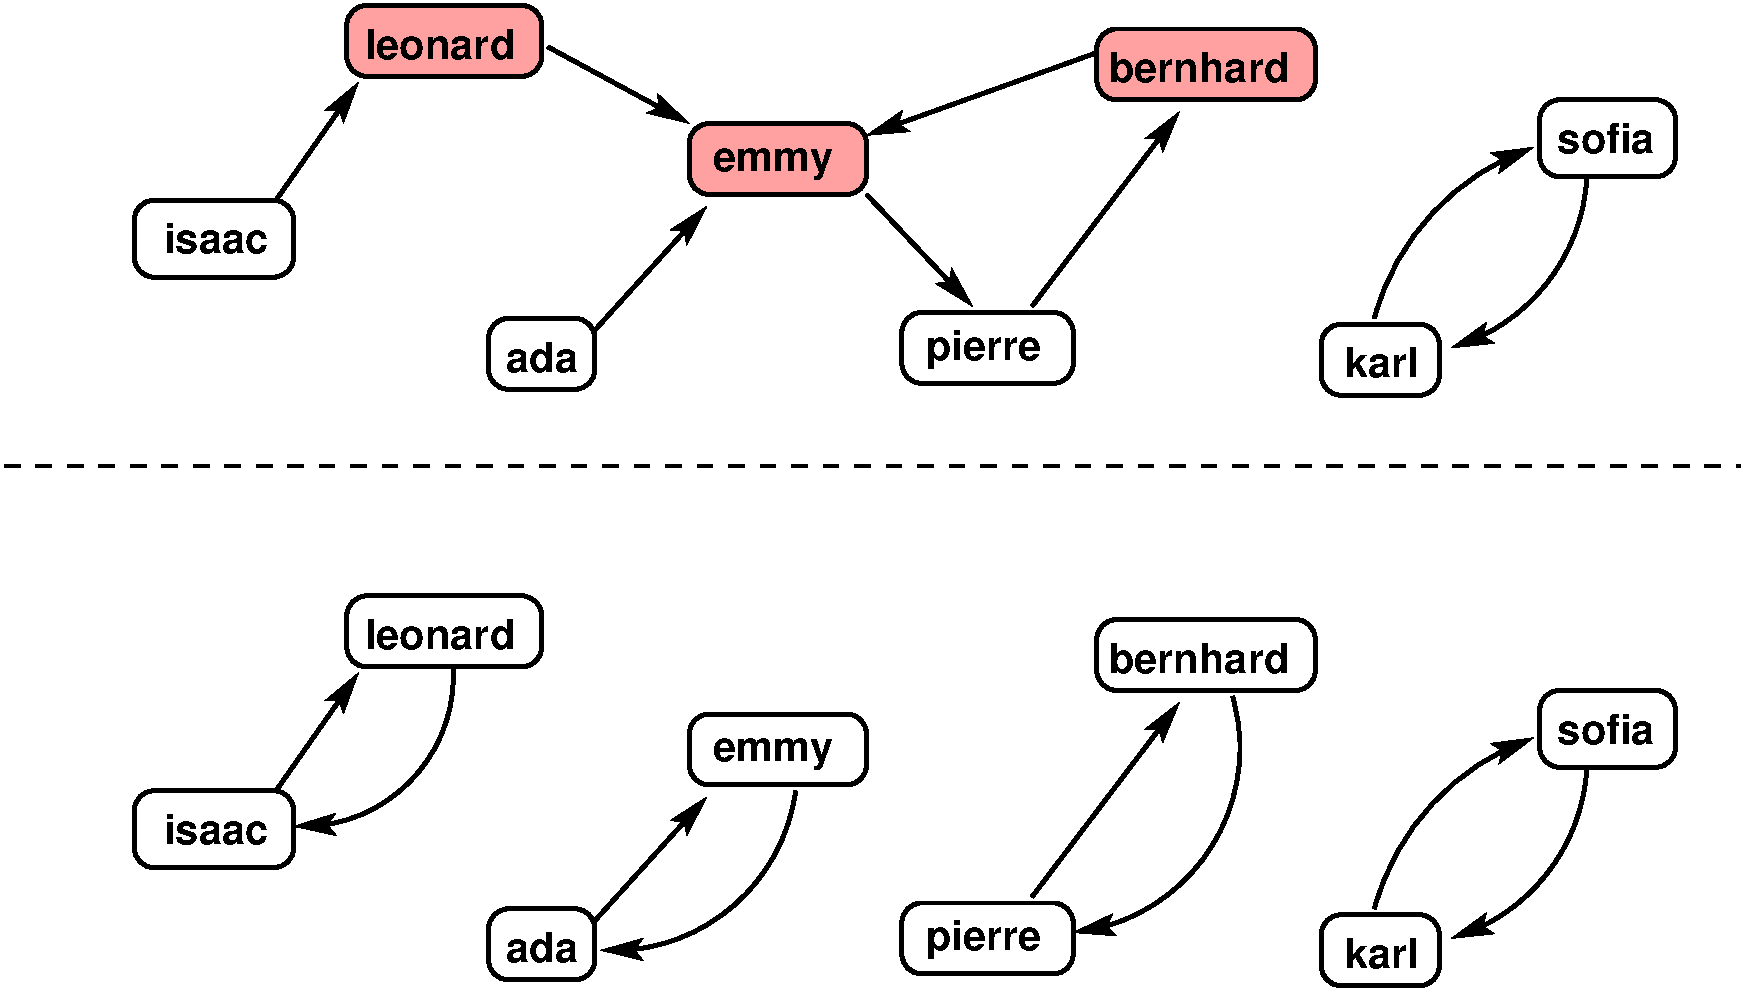
\includegraphics[width=0.5\textwidth]{polygonfig.pdf}
\end{center}

Первый пример проиллюстрирован на рисунке выше. Верхняя часть -- изначальная конфигурация отношений, где стрелка, ведущая от $s$ к $t$, указывает, что $s$ изначально любит $t$, а розовым цветом отмечены три персонажа, в которых нужно выстрелить стрелами любви, чтобы получить единственное оптимальное решение. Нижняя часть рисунка иллюстрирует результат.
%In the first example, there is a unique optimal solution: shoot 
%which consists of shooting \texttt{b}, \texttt{d} and \texttt{f} with love arrows, having them fall in love with \texttt{h}, \texttt{c} and \texttt{e}, respectively.

Во втором примере (который удовлетворяет условиям группы тестов 3) имеется несколько оптимальных решений. Одно из них -- выстрелить в \texttt{a}, \texttt{b} и \texttt{d},
и заставить их влюбиться в \texttt{b}, \texttt{a} и \texttt{c}, соответственно.

В третьем примере показан любовный треугольник, где, сколько ни стреляй, кто-нибудь всегда останется лишним.
